\documentclass[a4paper,10pt]{article}
\usepackage[utf8]{inputenc}
\usepackage[colorlinks,plainpages=false]{hyperref}

\setlength\parindent{0pt}
\usepackage[english]{babel}
\usepackage[dvinames]{xcolor}
\usepackage[compact,small]{titlesec}
\usepackage{booktabs}
\usepackage{multirow}
\usepackage{amsfonts,amsmath,amssymb}
\usepackage{marginnote}
\usepackage[top=1.8cm, bottom=1.8cm, outer=1.8cm, inner=1.8cm, heightrounded, marginparwidth=2.5cm, marginparsep=0.5cm]{geometry}
\usepackage{enumitem}
\setlist{noitemsep,parsep=2pt}
\newcommand{\highlight}[1]{\textcolor{kuleuven}{#1}}
\usepackage{pythonhighlight}
\usepackage{cleveref}
\usepackage{graphicx}
\graphicspath{{Pictures/}}
\usepackage{algorithmic}
\usepackage{tabularx}
\usepackage{bm}
\usepackage{subcaption}


\newcommand{\nextyear}{\advance\year by 1 \the\year\advance\year by -1}
\newcommand{\thisyear}{\the\year}
\newcommand{\deadlineGroup}{November 27, \thisyear{} at 16:00 CET}
\newcommand{\deadlineCode}{December 18, \thisyear{} at 16:00 CET}
\newcommand{\deadlineReport}{January 4, \nextyear{} at 16:00 CET}

\newcommand{\ReplaceMe}[1]{{\color{blue}#1}}
\newcommand{\RemoveMe}[1]{{\color{purple}#1}}

\setlength{\parskip}{5pt}

%opening
\title{Artificial Neural Networks: Exercise session 3}
\author{Stijn Staring (r0620003)}

\begin{document}
\fontfamily{ppl}
\selectfont{}

\maketitle


\section{Principal Component Analysis}
Principal component analysis is a method for dimensionality reduction. A principal component analysis uses the eigenvectors of the covariance matrix of the original data as principal components to conduct a linear transformation of the original data to a lower dimension. The eigenvectors that correspond to the largest eigenvalues are considered the most important principal components that determine data appearance the most.

\begin{equation}\label{eq:form1}
	\bm{z} = \bm{E}^T\bm{x}.
\end{equation}

In Eq. \ref{eq:form1}, $ \bm{x} $ is an original data point with dimensions $ \mathbb{R}^p $ and $ \bm{z} $ is the corresponding data point with reduced dimensions $ \mathbb{R}^q $. $ \bm{E}^T $ is the used transformation matrix with dimensions $ q \times p $ and with the $ q $ largest eigenvectors of the covariance matrix as rows. The new dimensions of the data point equals the amount of chosen eigenvectors that span the subspace. If all eigenvalues are distinct, $ \bm{E} $ is orthogonal and the original data point can be retrieved by multiplying Eq. \ref{eq:form1} by $ \bm{E} $ because of the orthogonality property: $ \bm{E}\cdot \bm{E}^{T} = \bm{I} $.\\

The first task performed is the comparison of the dimensionality reduction of random data in comparison to highly correlated data. It is found that there are less eigenvectors needed for the highly correlated data when the same RMSE is considered. The second task is to perform PCA on handwritten images of the digit 3 taken from the US Postal Service database. In this database every image consists out of $ 16 \times 16 $ pixels which is represented by an array of 256 floating numbers. The database consists out of a total of 500 images of the digit 3. When the mean array is calculated, also the mean digit 3 is obtained which is displayed in Figure \ref{fig:mean_three}. The covariance matrix is calculated for the data set and the eigenvalues derived are shown by Figure \ref{fig:50_largest_eigenvalues}. The influence of the amount of eigenvectors is demonstrated in Figure \ref{fig:increasing_eigenvectors}. When only one eigenvector is used, the reduced images are very similar. This means that the eigenvector with the largest eigenvalue focusses on the intrinsic shape of a 3. This means in what distinguishes a 3 from another number e.g. a 5. when more eigenvectors are used and the dimensionality of the spanned subspace increases, different variations of the digit 3 becomes clear. 

\begin{figure}[h!]
	\centering
	\begin{subfigure}[b]{0.49\textwidth}
		\centering
		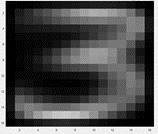
\includegraphics[width=0.55\linewidth]{mean_three.png}
		\caption{Mean image of digit 3}
		\label{fig:mean_three}
	\end{subfigure}
	\begin{subfigure}[b]{0.49\textwidth}
		\centering
		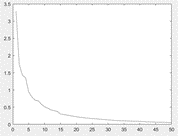
\includegraphics[width=0.6\linewidth]{50_largest_eigenvalues.png}
		\caption{Eigenvalues}
		\label{fig:50_largest_eigenvalues}
	\end{subfigure}
	\begin{subfigure}[b]{1.0\textwidth}
		\centering
		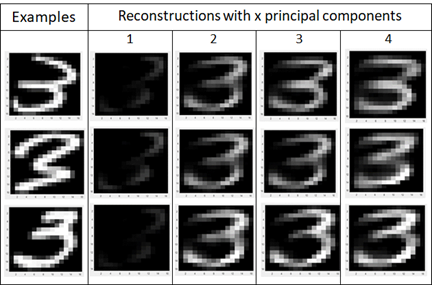
\includegraphics[width=0.4\linewidth]{reconstruction_x_principal_eigenvalues.png}
		\caption{Increasing amount of eigenvectors}
		\label{fig:increasing_eigenvectors}
	\end{subfigure}		
	\caption{Results of applying PCA on the US Postal Service database.}
	\label{fig:Results1}
\end{figure}

In Figure \ref{fig:Results2} the effect of the number of eigenvectors on the RMSE  used in the PCA, is investigated and the distribution of the sizes of the eigenvalues is shown. From Figure \ref{fig:Reconstruction_error1} it is concluded that when more eigenvectors are included, the representation error decreases because the dimensionality is less reduced. When the derivative of the function is assessed, it is found that the function decreases much faster at the beginning than at the end. This means that already by the use of a small amount of eigenvectors to span the subspace with a lower dimensionality, the reconstruction error can be significantly decreased and an already good reconstruction of the original data is possible. Figure \ref{fig:Reconstruction_error2} shows the cumulative sum of eigenvalues used in the PCA with on the x-axis the number of excluded eigenvalues starting from the largest. It is seen that a small amount of eigenvalues have large eigenvalues after which the size decreases rapidly. The plot is similar to Figure \ref{fig:Reconstruction_error1} and it can be concluded that the contribution of an eigenvector in reducing the RMSE corresponds to the size of the eigenvalue. This confirms what was concluded in Figure \ref{fig:Reconstruction_error1}, that already good representations of the digit 3 are possible with a small amount of eigenvectors. When Eq. \ref{eq:form1} is used without a dimensionality reduction, a very small reconstruction error equal to the default floating point precision in Matlab is found. 

\begin{figure}[h]
	\centering
	\begin{subfigure}[c]{0.49\textwidth}
		\centering
		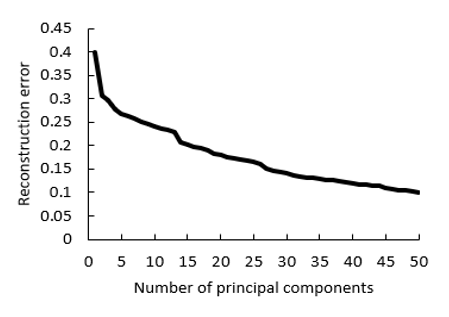
\includegraphics[width=0.85\linewidth]{Reconstruction_error1.png}
		\caption{}
		\label{fig:Reconstruction_error1}
	\end{subfigure}
	\begin{subfigure}[c]{0.49\textwidth}
		\centering
		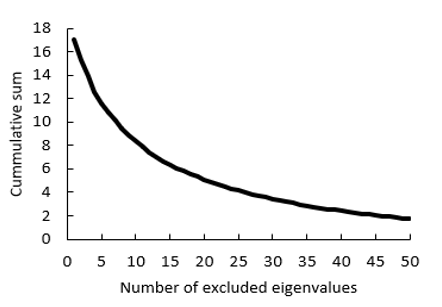
\includegraphics[width=0.8\linewidth]{Reconstruction_error2.png}
		\caption{}
		\label{fig:Reconstruction_error2}
	\end{subfigure}
	\caption{The influence of the amount of eigenvectors used.}
	\label{fig:Results2}
\end{figure}

\section{Stacked Autoencoders}
An autoencoder is an artificial neural network that learns efficient encodings of the original data. This is done by forcing the original data to be represented by only a limit amount of neurons causing a dimensionality reduction (encoding) after which the original data is reconstructed (decoding) and compared with the original inputs. When the outputs after decoding have a small reconstruction error, this means that the hidden layer that caused the dimensionality reduction, was able to identify the most important features determining the data appearance. This is similarly as the goal of the principal component analysis. Stacked autoencoders refers to the sequential use of autoencoders where the hidden layer of a previous autoencoder serves as input of a next one. Applications of dimensionality reduction making use of autoencoders are:
\begin{itemize}
	\item Image compression
	\item Denoising
	\item Feature extraction
\end{itemize}

Image compression is used when storing images on a hard drive and an autoencoder can also be applied when preprocessing to remove noise. Here, the focus will be on feature extraction. By forcing a dimensionality reduction, the most important features of the original data are extracted and this is also desired by each layer in a conventional neural network. Therefore, a deep neural network can be efficiently trained one layer at a time where this layer is the hidden layer in an autoencoder. Features will be combined to obtain new features in deeper layers of the network. The training approach used is greedy layer-wise training which means sequentially learning the layers of the deep neural network using autoencoders which is unsupervised. A softmax layer is added for classification which is trained in a supervised manner. Finally, fine tuning is conducted which means that the total deep neural network is constructed and trained using labelled images. Next, the influence of different parameters is discussed. 

\subsection{MaxEpochs}
During training of the autoencoder, the softmax layer and fine-tuning, the general rule of overfitting applies which states that: when a high number of epochs are trained, the training error will decrease but the validation error will start to increase at a certain point in time. The point where the validation error starts to increase corresponds to the moment in time that the network stops learning general features from the inputs. Because it starts to remember specific aspects of the training data, this will not be general anymore and the error on unseen inputs i.e. the validation set, will increase. A suitable solution is to set a high value for MaxEpochs while monitoring the error on the validation set. This method is called early stopping and is by default applied in Matlab when applying supervised learning. 

\subsection{Number of hidden units}
The tradeoff that has to be made when choosing the amount of hidden neurons in the autoencoder is twofold. When the amount of neurons is selected too large, with as maximum equal to the dimensionality of the inputs, the dimensionality reduction is only small and the autoencoder is not pushed towards making satisfactory generalizations. This means that the learned hidden layer is very input specific with as extreme case that it just learns the identity function and no features are extracted. The reconstruction error will in this case be zero. On the other side, when a small amount of hidden units are selected, a very large dimensionality reduction is forced which causes the extracted features to be not representative for the inputs. This will give a large reconstruction error. The most suitable amount of hidden units is in between the two extremes and problem specific. The amount of units chosen in the softmax layer corresponds to the amount of classes using an one hot encoding.

\subsection{Number of layers}
When more layers are used in the deep neural network the expressiveness of the model increases. Features will be combined to obtain new features in deeper layers of the network. Especially, when a model has a high expressiveness, extra care should be taken with overfitting. The increase of the amount of layers didn't give much improvement to the classification results. This indicates that the most relevant features used when classifying are already extracted in the first layer.\\ 

\subsection{Parameter tuning}
The default settings give already very satisfactory results and have before fine-tuning a correct classification in $ 87.04\% $  and after fine-tuning in $ 99.74\% $ of the cases. Despite this, a small parameter search was conducted which varied the amount of epochs, hidden units, and hidden layers. Every combination of values for the parameters is repeated 3 times in order to reduce the dependency of the results on the random weight initialisations. The best average run found has a correct classification of $ 98.88\% $ after fine-tuning.\\

Fine-tuning causes an additional increase of the correctness of classification and is necessary if the the method using autoencoders wants to outperform the conventional way of training neural networks with default parameter values, which achieved a classification accuracy of $ 95.36\% $ and $ 97.24\%$ for respectively the use of one and two hidden layers. Fine-tuning is important because now the network is seen as a whole and the final classification error influences all the layers simultaneously by making use of back propagation. In comparison, first every hidden layer and softmax layer is trained individually and afterwards stacked together. Only one hidden layer is needed together with 100 hidden units and 400 epochs to outperform the conventional neural networks. An average classification correctness was found of $ 98.88\% $ and fine-tuning only leads to an improvement of $ 0.28\% $. 

\section{Convolutional Neural Network}
When processing images to extract features, every pixel of the image is an individual input. When high resolution images are processed, a lot of inputs are given to a conventional neural network and the amount of weights that should be learned blows up. This has as consequence that the use of conventional neural networks is not possible anymore due to the high calculation load. In order to deal with this, two assumptions are made. The first assumption is stationarity or translation invariance, which means that whatever patch of the image is assessed, the network should respond similarly on the use of feature detectors. For example, if the feature that is looked for are edges, it is assumed that an edge is perceived the same everywhere in the image. The second assumption is the locality principle which means that only a small neighbourhood of the image is assessed at a time. This is a suitable assumption for images, because a pixel is much more related to pixels which are close. Because of these two assumptions a CNN can be developed that captures local spatial patterns in the data and an explosion of the amount of weights is avoided.
A CNN can learn rich feature representations for 2D images and can therefore be applied as preprocessing tool to extract important features. The building blocks of a CNN network is the altering use of convolutional layers, Relu layers and pooling layers.\\


The convolution layer specifies an amount of feature detectors with a certain size. A feature detector is in literature also called a filter or convolutional kernel. Every kernel conducts a convolutional operation with the original image and outputs a feature map. A feature map shows were in the original image the kernel has found a good match with the feature that it is focussing on. When going deeper in the CNN, the features that will be detected will become more advanced. For example in the first layer features will be edges and later on become parts of real objects. For every kernel, a feature map is calculated which shows were in the picture a good match is found. After the convolution layers, Relu layers are applied that set all the negative values in the feature map equal to zero.\\

In the pooling layer, dimensionality of the feature map is reduced by making use of a max value or average value operation. The advantage of using max value is that it adds additional non-linearity with respect to taking the average value. A pooling windows traverses the feature map with a certain stride (step in number of pixels taken by the window) and calculates in the case of max value, the max value for each window. Afterwards, an in dimensionality reduced version of the feature map will be left.\\

After the altering convolutional, Relu and pooling layers a fully connected network is added to use the extracted features as inputs for classification. The total network is trained in a supervised manner and therefore the error with the observations can be back propagated through the whole network to tune the weights in the fully connected layers and to define the features that will be looked for in the kernels of the convolutional layers. The weights that are learned in the kernel are shared during their application in the conventional layer. Convolutions performed are easy to parallelize across GPU cores, which speeds up calculations. Finally, it is noted that striding can also be used for the window of the kernel and padding can be applied to influence the dimensionality of the output of a convolution or pooling layer. Channel normalization layers are used to counteract vanishing gradients.\\
When inspecting layer 2, which corresponds to the first convolution layer, it is seen that there are 96 separate kernels specified, each with dimensions of $ 11 \times 11 \times 3 $. All these kernels are separately applied on the image with dimensions $ 227 \times 227 \times 3 $ to form feature maps. The third dimension corresponds to the colour specification according to the RGB values. A stride of 4 in the horizontal and vertical direction is used when the kernel traverses the image. Because the CNN is already trained, the weights in the kernel functions correspond to the learned features where will be looked for in the image. The weights of the kernel are obtained by making use of back propagation.\\
The dimensions of the inputs only change after a convolution layer or pooling layer and from every window of values only one remains. Following formulas can be applied when identical horizontal and vertical dimensions for the kernel size and inputs is used, padding $ Pa $ is applied the same for all edges, $ X $ the new dimension, $ I $ the original dimension, $ K $ the kernel window dimension,$  P $ the pooling window dimension and $ S $ the stride 

\begin{subequations}
	\begin{equation}
		X = \frac{(I + 2Pa -K)}{S} + 1,
	\end{equation} 
	\begin{equation}
			X = \frac{(I+2Pa-P)}{S} + 1.
	\end{equation}   
\end{subequations}

The inputs for the second convolution layer are therefore 96 feature maps with dimensions $ 27 \times 27 \times 1$ and the inputs before the fully connected layers are 256 feature maps with dimensions $ 6 \times 6 \times 1$. The original image is broken down a large amount of small feature maps. The advantage of a CNN wit respect to a conventional fully connected neural network is as discussed below the dimensionality reduction done by extracting important features which are then feeded to a fully connected neural network.\\
During te










%\begin{table}
%	\centering
%	\begin{tabular}{@{}clr@{}} \toprule
%		\textbf{Attractor} & \textbf{Point} & \textbf{Stability}\\\midrule
%		Attractor $ 1 $ & $ [1;1] $ & Stable\\
%		Attractor $ 2 $ & $ [-1;-1] $ & Stable\\
%		Attractor $ 3 $ & $ [1;-1] $ & Stable\\
%		Attractor $ 4 $ & $ [-1;1] $ & Stable\\
%		Attractor $ 5 $ & $ [0;0] $ & Unstable\\
%		Attractor $ 6 $ & $ [0;1] $ & Unstable\\
%		Attractor $ 7 $ & $ [0;-1] $ & Unstable\\
%		Attractor $ 8 $ & $ [1;0] $ & Unstable\\
%		Attractor $ 9 $ & $ [-1;0] $ & Unstable\\\bottomrule
%	\end{tabular}
%	\caption{Overview of the different attractor points found in a 2D plane.}
%	\label{tab:att}
%\end{table}

\bibliographystyle{abbrv}
%\bibliography{ANN1}

\end{document}
